\documentclass[11pt]{article}
\usepackage{geometry}                % See geometry.pdf to learn the layout options. There are lots.
\geometry{letterpaper}                   % ... or a4paper or a5paper or ... 
%\geometry{landscape}                % Activate for for rotated page geometry
%\usepackage[parfill]{parskip}    % Activate to begin paragraphs with an empty line rather than an indent
\usepackage{graphicx}
\usepackage{amssymb}
\usepackage{epstopdf}
\usepackage{fixltx2e}			%provides \textsubscript
\DeclareGraphicsRule{.tif}{png}{.png}{`convert #1 `dirname #1`/`basename #1 .tif`.png}


%%
%% TIKZ for drawing DAGs (not sure how much of the below is necessary)
%%

\usepackage{tikz}
\usepackage{tkz-graph}
\usetikzlibrary{shapes,arrows}

\newcommand{\entrynode}[1]{
  \SetVertexNormal[Shape      = circle,
                   FillColor  = black,
                   LineWidth  = 0pt,
                   MinSize    = 0pt]
  \Vertex[L={\tiny\,}]{#1}
  \SetVertexNormal[Shape      = circle,
                   FillColor  = white,
                   LineWidth  = 2pt]
}

\SetUpEdge[lw         = 1.5pt,
           color      = black,
           labelcolor = white,
           labeltext  = red,
           labelstyle = {sloped,draw,text=blue}]

\tikzset{node distance = 2cm}




\title{Anonymity in XIA: Developer Tools and User Control}
\author{Nicolas Feltman and David Naylor}
\date{}                                           


\begin{document}
\maketitle
\section{Introduction}
\subsection{Anonymity}
\subsection{XIA}


\section{Levels of Anonymity}


\section{Approach: Proxies}
The first approach we will discuss for providing anonymity is proxies.  The basic idea behind a proxy is for a service requester to route all of its communications with a service provider through an auxiliary party called a proxy.  Since the service provider only ever interacts with the proxy and never with the server requester directly, it does not need to know the machine address (i.e. identity) of the requester.

In this section we will discuss one possible way to implement a proxy protocol for persistent connections.  

\subsection{Proxy Addresses}

One key feature of our proxy protocol design is including the proxy's address with the address of the service provider in a single DAG.  This means that from the point of view of a client program developer, the use of a proxy can be expressed entirely within the service provider's address DAG.  Although we provide an anonymous communication API, it is little more than syntactic sugar over the standard library.  Although we considered introducing a new principle type for proxy services, we found that they could be expressed sufficiently with the standard service principle type.  The DAG in figure ({\bf HELP I DON'T KNOW HOW TO DO FIGURES}) represents communication with the end service SID\textsubscript{E} via the proxy SID\textsubscript{P}, with backup paths for both.  We do not cover in this document how the proxy's DAG is resolved.

\begin{center}
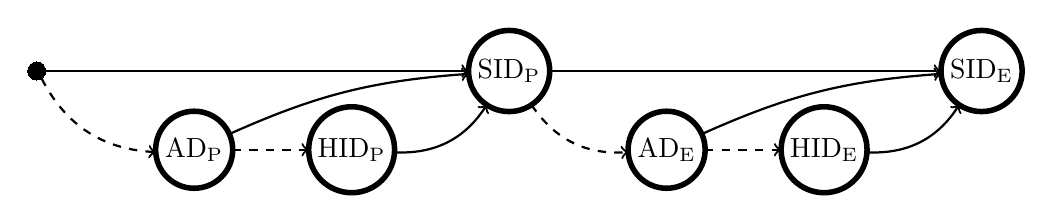
\begin{tikzpicture}
  \entrynode{A}
  \Vertex[x=6,y=0,L=SID\textsubscript{P}]{B}
  \Vertex[x=2,y=-1,L=AD\textsubscript{P}]{C}
  \Vertex[x=4,y=-1,L=HID\textsubscript{P}]{D}
  \Vertex[x=12,y=0,L=SID\textsubscript{E}]{E}
  \Vertex[x=8,y=-1,L=AD\textsubscript{E}]{F}
  \Vertex[x=10,y=-1,L=HID\textsubscript{E}]{G}
  \tikzstyle{EdgeStyle}=[->]
  \Edge(A)(B)
  \tikzstyle{EdgeStyle}=[dashed, bend right, ->]
  \Edge(A)(C)
  \tikzstyle{EdgeStyle}=[bend left=10, ->]
  \Edge(C)(B)
  \tikzstyle{EdgeStyle}=[dashed, ->]
  \Edge(C)(D)
  \tikzstyle{EdgeStyle}=[bend right, ->]
  \Edge(D)(B)
  \tikzstyle{EdgeStyle}=[->]
  \Edge(B)(E)
  \tikzstyle{EdgeStyle}=[dashed, bend right, ->]
  \Edge(B)(F)
  \tikzstyle{EdgeStyle}=[bend left=10, ->]
  \Edge(F)(E)
  \tikzstyle{EdgeStyle}=[dashed, ->]
  \Edge(F)(G)
  \tikzstyle{EdgeStyle}=[bend right, ->]
  \Edge(G)(E)
\end{tikzpicture}
\end{center}

\subsection{Protocol}

This version of the protocol assumes that the client application does not need to communicate any connection parameters with proxy.  The client begins by resolving DAGs for the proxy and for the end service.  Let the proxy service have the public address SID\textsubscript{P} and the end service have the address SID\textsubscript{E}. Let the client application be running on a host H\textsubscript{C} with the local service identifier SID\textsubscript{A}.  It sends the initial packet with the following destination and source addresses (backup paths omitted):

\begin{center}
    \begin{tabular}{ | l | l |} \hline
    	Dst & Src \\ 
	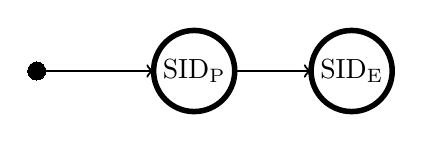
\begin{tikzpicture}
	\entrynode{A}
	\Vertex[x=2,y=0,L=SID\textsubscript{P}]{P}
	\Vertex[x=4,y=0,L=SID\textsubscript{E}]{E}
	\tikzstyle{EdgeStyle}=[->]
	\Edge(A)(P)
	\tikzstyle{EdgeStyle}=[->]
	\Edge(P)(E)
	\end{tikzpicture} &
	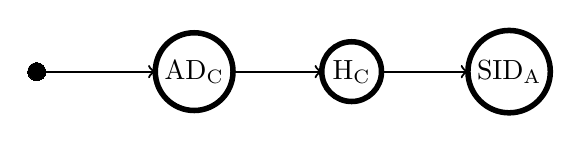
\begin{tikzpicture}
	\entrynode{B}
	\Vertex[x=2,y=0,L=AD\textsubscript{C}]{A}
	\Vertex[x=4,y=0,L=H\textsubscript{C}]{H}
	\Vertex[x=6,y=0,L=SID\textsubscript{A}]{S}
	\tikzstyle{EdgeStyle}=[->]
	\Edge(B)(A)
	\tikzstyle{EdgeStyle}=[->]
	\Edge(A)(H)
	\tikzstyle{EdgeStyle}=[->]
	\Edge(H)(S)
	\end{tikzpicture}
    \\ \hline
    \end{tabular}
\end{center}

Upon receiving this initial packet, the proxy service chooses a particular machine, henceforth H\textsubscript{P}, to handle this connection.  If AD\textsubscript{C}.HID\textsubscript{C}.SID\textsubscript{A} is not already in this machine's rerouting table, the proxy creates a new local service ID, SID\textsubscript{T} (for tunnel), and adds this pair to its rerouting table.  The machine then forwards the intial packet with the following destination and source addresses:

\begin{center}
    \begin{tabular}{ | l | l |} \hline
    	Dst & Src \\ 
	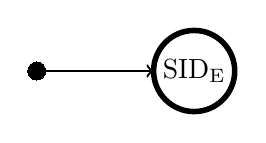
\begin{tikzpicture}
	\entrynode{A}
	\Vertex[x=2,y=0,L=SID\textsubscript{E}]{E}
	\tikzstyle{EdgeStyle}=[->]
	\Edge(A)(E)
	\end{tikzpicture} &
	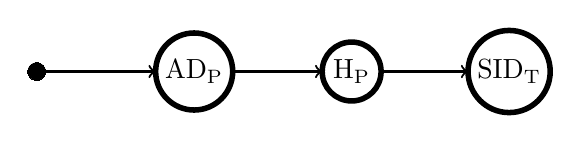
\begin{tikzpicture}
	\entrynode{B}
	\Vertex[x=2,y=0,L=AD\textsubscript{P}]{A}
	\Vertex[x=4,y=0,L=H\textsubscript{P}]{H}
	\Vertex[x=6,y=0,L=SID\textsubscript{T}]{S}
	\tikzstyle{EdgeStyle}=[->]
	\Edge(B)(A)
	\tikzstyle{EdgeStyle}=[->]
	\Edge(A)(H)
	\tikzstyle{EdgeStyle}=[->]
	\Edge(H)(S)
	\end{tikzpicture}
    \\ \hline
    \end{tabular}
\end{center}

The end service is not aware that it is communicating via a proxy.  It chooses a machine, H\textsubscript{E}, to handle this connection, and responds with the following packet header:

\begin{center}
    \begin{tabular}{ | l | l |} \hline
    	Dst & Src \\
	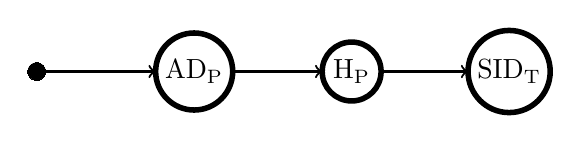
\begin{tikzpicture}
	\entrynode{B}
	\Vertex[x=2,y=0,L=AD\textsubscript{P}]{A}
	\Vertex[x=4,y=0,L=H\textsubscript{P}]{H}
	\Vertex[x=6,y=0,L=SID\textsubscript{T}]{S}
	\tikzstyle{EdgeStyle}=[->]
	\Edge(B)(A)
	\tikzstyle{EdgeStyle}=[->]
	\Edge(A)(H)
	\tikzstyle{EdgeStyle}=[->]
	\Edge(H)(S)
	\end{tikzpicture} &
	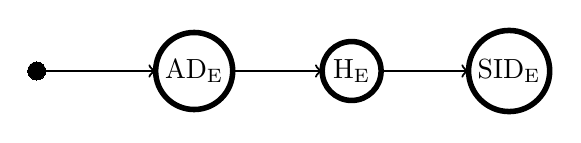
\begin{tikzpicture}
	\entrynode{B}
	\Vertex[x=2,y=0,L=AD\textsubscript{E}]{A}
	\Vertex[x=4,y=0,L=H\textsubscript{E}]{H}
	\Vertex[x=6,y=0,L=SID\textsubscript{E}]{S}
	\tikzstyle{EdgeStyle}=[->]
	\Edge(B)(A)
	\tikzstyle{EdgeStyle}=[->]
	\Edge(A)(H)
	\tikzstyle{EdgeStyle}=[->]
	\Edge(H)(S)
	\end{tikzpicture}
    \\ \hline
    \end{tabular}
\end{center}

The proxy, in the interest of keeping minimal state, does not remember this source address but instead sends it back to the client in what the client sees as the first response:

\begin{center}
    \begin{tabular}{ | l |} \hline
    	Dst \\ 
	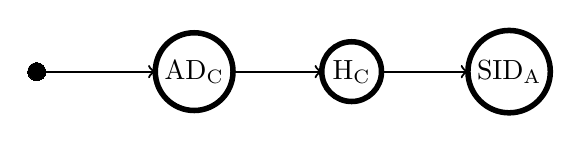
\begin{tikzpicture}
	\entrynode{B}
	\Vertex[x=2,y=0,L=AD\textsubscript{C}]{A}
	\Vertex[x=4,y=0,L=H\textsubscript{C}]{H}
	\Vertex[x=6,y=0,L=SID\textsubscript{A}]{S}
	\tikzstyle{EdgeStyle}=[->]
	\Edge(B)(A)
	\tikzstyle{EdgeStyle}=[->]
	\Edge(A)(H)
	\tikzstyle{EdgeStyle}=[->]
	\Edge(H)(S)
	\end{tikzpicture} \\ \hline
	Src \\ 
	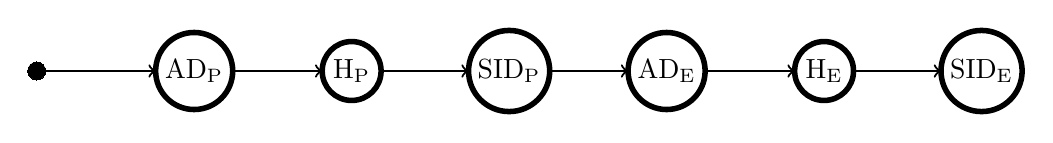
\begin{tikzpicture}
	\entrynode{B}
	\Vertex[x=2,y=0,L=AD\textsubscript{P}]{A}
	\Vertex[x=4,y=0,L=H\textsubscript{P}]{H}
	\Vertex[x=6,y=0,L=SID\textsubscript{P}]{S}
	\Vertex[x=8,y=0,L=AD\textsubscript{E}]{A2}
	\Vertex[x=10,y=0,L=H\textsubscript{E}]{H2}
	\Vertex[x=12,y=0,L=SID\textsubscript{E}]{S2}
	\tikzstyle{EdgeStyle}=[->]
	\Edge(B)(A)
	\tikzstyle{EdgeStyle}=[->]
	\Edge(A)(H)
	\tikzstyle{EdgeStyle}=[->]
	\Edge(H)(S)
	\tikzstyle{EdgeStyle}=[->]
	\Edge(S)(A2)
	\tikzstyle{EdgeStyle}=[->]
	\Edge(A2)(H2)
	\tikzstyle{EdgeStyle}=[->]
	\Edge(H2)(S2)
	\end{tikzpicture}
    \\ \hline
    \end{tabular}
\end{center}

The client then binds to this source DAG, sending all future communications to it.  Thus, the client continues communicating with the host via the proxy, the proxy swaps references to HID\textsubscript{C}.SID\textsubscript{A} with HID\textsubscript{P}.SID\textsubscript{T}, and the end service thinks it is maintaining a persistent connection with HID\textsubscript{P}.SID\textsubscript{T}.  

\section{Approach: Temporary Service IDs}



\section{An API for Developers}
As we have discussed above, XIA allows for simple, if not elegant, ways to employ techniques for anonymization. For instance, we explored how an application can achieve fine-grain control over the use of a proxy service through DAG manipulation. We also proposed the use of temporary SIDs as pseudonyms.

Both of these strategies incorporate anonymity by leveraging core features of XIA. Thus, it is both possible and useful to a standard set of tools implementing these techniques to application developers --- it would be silly for each developer to implement his/her own functions for adding a proxy service to all outgoing DAGs, for example.

We have implemented these tools in the form of the XAnonSocket API, an extension to the XSocket API. (The XSocket API, as the name suggests, allows developers to communicate with sockets over XIA, much like network applications today use TCP or UDP sockets.) The XAnonSocket API allows developers to specify how they want to achieve anonymity (i.e., by routing traffic through a proxy of their choice) just once, after which they can send packets using the specified service with no extra effort. In \S~\ref{sec:api-interface} we present the interface of the XAnonSocket API.

\subsection{API Interface}
\label{sec:api-interface}

\begin{center}
	\begin{tabular}{l p{7cm}}
	\textbf{Function} 	&	\textbf{Description}\\
	\hline
	\texttt{XAnonSocket()} & Creates an anonymous XIA socket\\
	\texttt{XAnonRegisterAnonymizer(sock, dag)} & Specifies the DAG of an anonymization (e.g., proxy) service all packets sent through \texttt{sock} should be routed through\\
	\texttt{XAnonUseTempSID(sock, duration)} & Future packets should be sent from a temporary SID with HID elided. A new SID is generated after \texttt{duration} seconds\\
	\texttt{XAnonConnect(sock, dag)} & Connect to \texttt{ddag} with current anonymization settings\\
	\texttt{XAnonSend(sock, payload)} & Sends a packet with current anonymization settings\\
	\texttt{XAnonGetStatus(sock)} & Retrieves the current anonymization settings for \texttt{sock}\\
	\hline
	\end{tabular}
\end{center}


\section{Example Application: Web Browser}

\end{document}  